\documentclass{article}


%%%%%%%%%%%%%%%%%%%%%%%%%%%%%%%%%%%%%%%%%%%%%%%%%%%%%%%%%%%%%%%%%%%%%%%%%
\pagestyle{plain}                                                      %%
%%%%%%%%%% EXACT 1in MARGINS %%%%%%%                                   %%
\setlength{\textwidth}{6.5in}     %%                                   %%
\setlength{\oddsidemargin}{0in}   %% (It is recommended that you       %%
\setlength{\evensidemargin}{0in}  %%  not change these parameters,     %%
\setlength{\textheight}{8.5in}    %%  at the risk of having your       %%
\setlength{\topmargin}{0in}       %%  proposal dismissed on the basis  %%
\setlength{\headheight}{0in}      %%  of incorrect formatting!!!)      %%
\setlength{\headsep}{0in}         %%                                   %%
\setlength{\footskip}{.5in}       %%                                   %%
%%%%%%%%%%%%%%%%%%%%%%%%%%%%%%%%%%%%                                   %%
\newcommand{\required}[1]{\section*{\hfil #1\hfil}}                    %%
\renewcommand{\refname}{\hfil References Cited\hfil}                   %%
\bibliographystyle{plain}                                              %%
%%%%%%%%%%%%%%%%%%%%%%%%%%%%%%%%%%%%%%%%%%%%%%%%%%%%%%%%%%%%%%%%%%%%%%%%%

\usepackage{graphicx}

\pagestyle{empty}

\begin{document}

\large

\vbox{}
\begin{figure}[!ht]
%\hspace{-4mm}

\includegraphics[width=8cm]{img/logo.png}
\vspace{16mm}
\end{figure}

\begin{figure}[!ht]
\begin{center}
%\hspace{-4mm}
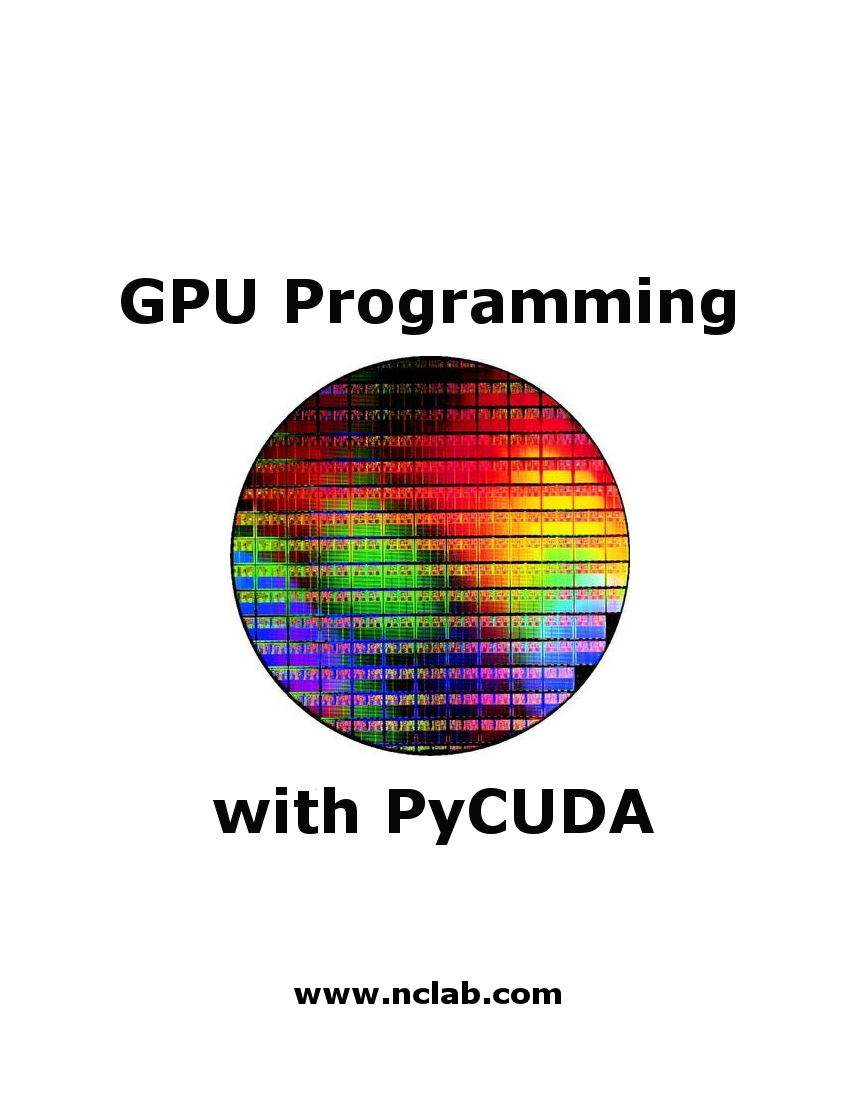
\includegraphics[width=10cm]{img/cuda-frontpage.png}
\vspace{18mm}
\end{center}
\end{figure}

\centerline{\Huge \bf GPU Computing with PyCUDA}

\vfill

\centerline{\Large www.nclab.com}

\newpage

%%%%%%%%%%%%%%%%%%%%%%%%%%%%%%%%%%%%%%%%%%%%%%%%%%%%%%%%%%%%%%%%%%%%%%%%%



\section*{}


%\subsection*{Acknowledgement}
%This publication was created with the help of numerous freely 
%available web resources and tutorials related to Python, Scipy,
%Numpy, Pylab, Matplotlib, Sympy and other projects.

\normalsize

\newpage
%{\ }
\setcounter{tocdepth}{2}
\tableofcontents
%\pagestyle{plain}

\newpage

\pagestyle{plain}
\setcounter{page}{1}


%%%%%%%%%%%%%%%%%%%%%%%%%%%%%%%%%%%%%%%%%%%%%%%%%%%%%%%%%%%%%%%%%%%%%%%%%
\newpage

\pagestyle{plain}

\section{GPU, CUDA, and PyCUDA}

{\em Graphical Processing Unit (GPU)} computing belongs to the newest trends in
Computational Science worldwide. The reason for its attractivity is mainly 
the high computing power of modern graphics cards. For example, the 
Nvidia Tesla C2070 GPU computing processor shown in Fig. \ref{fig:tesla} 
has 448 cores and 6 GB of memory, with peak performance of 1030 and 515 
GFlops in single and double precision arithmetic, respectively.


\begin{figure}[!ht]
\begin{center}
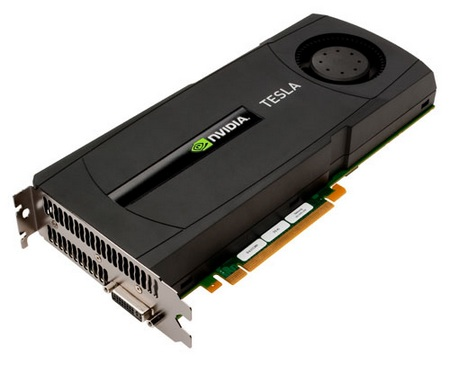
\includegraphics[width=0.5\textwidth]{img/tesla.png}
\caption{Nvidia Tesla C2070.}
\label{fig:tesla}
\end{center}
\end{figure}
\noindent
These cards are still quite expensive -- the card shown in Fig. \ref{fig:tesla} costs 
around \$2,000 as of March 2012. Therefore, GPU computing may not be easily accessible 
to all who would like to experiment with it. This was the main reason why we decided to 
include GPU programming in NCLab. 

{\em Compute Unified Device Architecture (CUDA)} is a parallel computing architecture 
developed by Nvidia for graphics processing. CUDA is the computing engine in 
Nvidia GPUs that is accessible to software developers through variants of 
industry standard programming languages.

CUDA bindings are available in many high-level languages including Fortran,
Haskell, Lua, Ruby, Python and others. We are specifically interested 
in Python bindings (PyCUDA) since Python is the main programming language 
of NCLab. PyCUDA was written by Andreas Kl\"ockner (Courant Institute 
of Mathematical Sciences, New York University).





\section{PyCUDA in NCLab}

In order to make the most of this tutorial, we invite the 
reader to create an account in NCLab and log in. More instructions 
on how to do this are given at the beginning of the introductory 
tutorial "Meet Your New Graphing Calculator" that is available in 
PDF via a link on NCLab home page {\tt http://nclab.com}. \\

\noindent
After login, you will see a desktop with several icons on it,
as shown in Fig. \ref{fig:desktop}. 

\begin{figure}[!ht]
\begin{center}
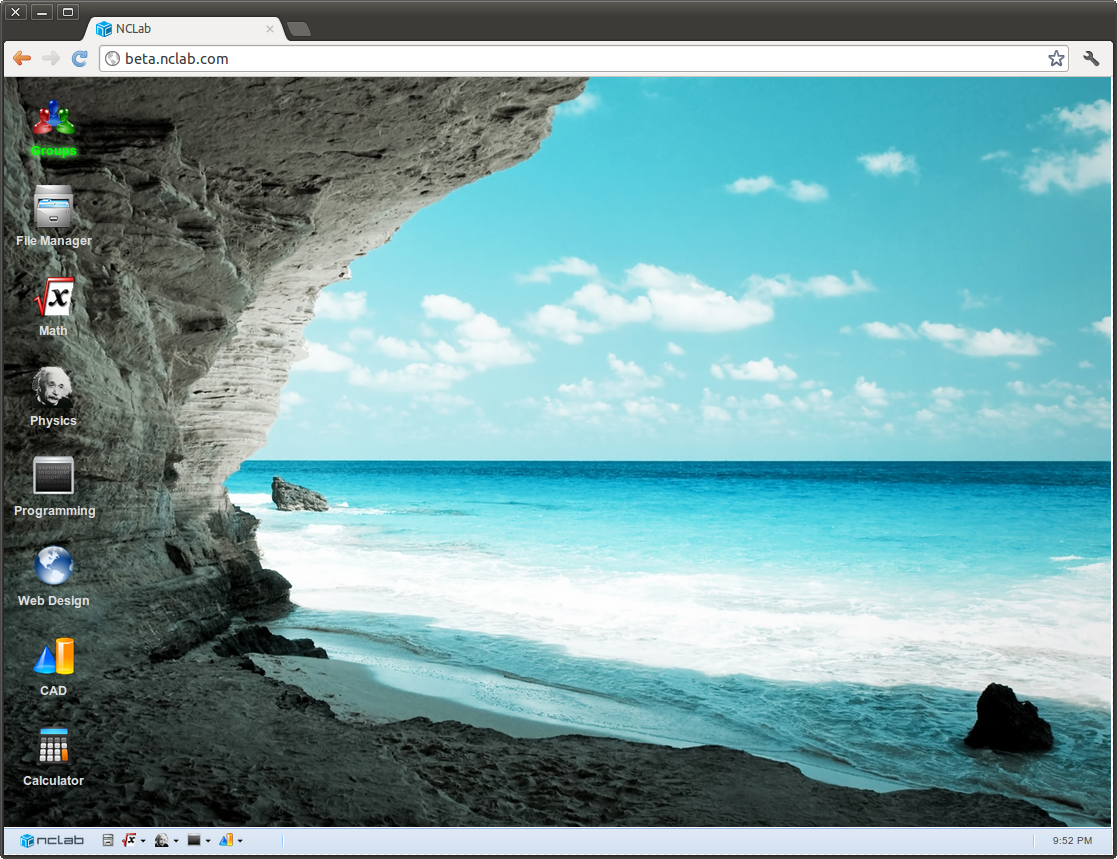
\includegraphics[width=0.9\textwidth]{img/desktop.png}
\end{center}
%\vspace{-2mm}
\caption{NCLab desktop after login.}
\label{fig:desktop}
\end{figure}

\subsection{Cloning Displayed Projects}

All examples that we are going to work with in the following are also available 
as Displayed Projects. This means that you can clone them by launching the File
Manager, going to the {\em Project} menu, and clicking on {\em Clone}. This will launch 
a window with many displayed projects from various areas of programming,
math and computing. Look for projects whose names start with "PyCUDA - Tutorial".
After you locate a project that you would like to clone, click on it,
and then click on the button {\em Clone} at the bottom of the window. This will
create exact copy of that project in your account, and you can open it 
by clicking on it in the File Manager. You can change the project in any way 
you like, the changes will not affect the original Displayed Project. 


\subsection{Launching a new PyCUDA project}

Alternatively, you can start by launching an empty PyCUDA project through 
{\em Programming} $\rightarrow$ {\em PyCUDA}, as shown in Fig. \ref{fig:pycuda}.

\newpage


\begin{figure}[!ht]
\begin{center}
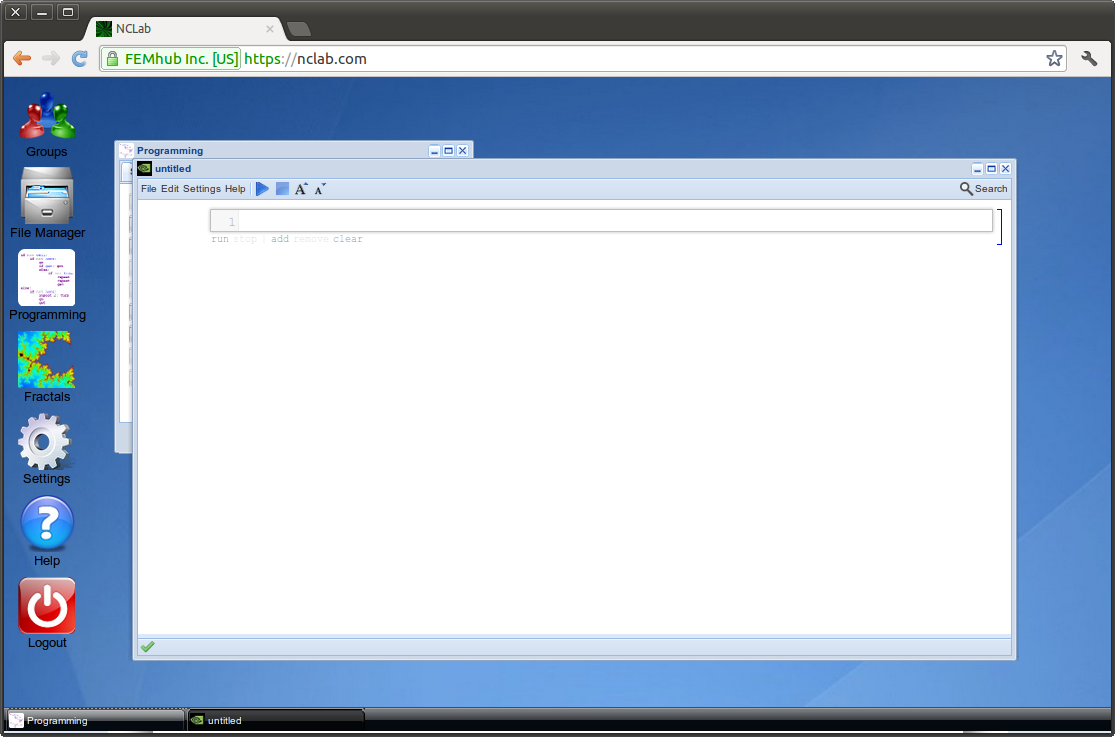
\includegraphics[width=0.9\textwidth]{img/pycuda.png}
\end{center}
%\vspace{-2mm}
\caption{Launching a new PyCUDA project.}
\label{fig:pycuda}
\end{figure}
\noindent


\section{Hello World!}\label{sec:hello}

Let us demonstrate the PyCUDA workflow on a very simple example that 
generates a 4x4 random array on the CPU, sends it to the GPU where 
all entries are doubled in parallel, and then the result is sent 
back to the CPU and displayed. 

\subsection{Import and initialize PyCUDA}

Either clone the displayed project "PyCUDA - Tutorial - 01" or type the following 
code into a newly opened PyCUDA project:
\begin{verbatim}
import pycuda.driver as cuda
import pycuda.autoinit
from pycuda.compiler import SourceModule
\end{verbatim}
Here, {\tt pycuda.autoinit} serves for automatic initialization, context creation, 
and cleanup. The {\tt SourceModule} is where a (usually short) C-like code for the 
GPU is to be written. More about this will be said in a moment. 

\subsection{Generate your data}

Numpy arrays (large matrices) are the most frequently used data type to be 
transferred to a GPU. So, let us import Numpy and generate a 4x4 random array:
\begin{verbatim}
import numpy
a = numpy.random.randn(4, 4)
\end{verbatim}

\subsection{Convert your data to single precision if needed}

The array created in Step 2 contains double precision numbers and the GPU units in NCLab can 
process them (in general, older units cannot). However, if accuracy does not matter so much 
and we want this job done faster, we can convert the double precision numbers into single precision 
anyway:

\begin{verbatim}
a = a.astype(numpy.float32)
\end{verbatim}

\subsection{Transfer your data to GPU}

First we need to allocate memory on the device using the CUDA driver:
\begin{verbatim}
a_gpu = cuda.mem_alloc(a.nbytes)
\end{verbatim}
Then we can transfer the Numpy array to the device:

\begin{verbatim}
cuda.memcpy_htod(a_gpu, a)
\end{verbatim}
Notably, the array {\tt a\_gpu} is one-dimensional and on the device we need to 
handle it as such.

\subsection{Compile your parallel C code and load it on the GPU}

To keep the Hello World example simple, let us write a program that just doubles 
each entry of the (now one-dimensional) array:
\begin{verbatim}
mod = SourceModule("""
  __global__ void doublify(float *a)
  {
    int idx = threadIdx.x + threadIdx.y * 4;
    a[idx] *= 2;
  }
  """)
\end{verbatim}
The thing that makes this code interesting is that {\em it only gets executed
once} -- in 16 different threads. Both the variables {\tt threadIdx.x} and {\tt threadIdx.y}
contain indices between $0$ and $3$, and the pair is different for each thread. 

\subsection{Call your function}

The code from Step 5 is compiled with the {\tt nvcc} compiler automatically. 
If there are no errors, we can obtain a pointer to the compiled function:

\begin{verbatim}
func = mod.get_function("doublify")
\end{verbatim}
Then we can call it with {\tt a\_gpu} as the argument, and the block size of 4x4:

\begin{verbatim}
func(a_gpu, block = (4, 4, 1))
\end{verbatim}

\subsection{Fetch your results from the GPU}

To fetch the result, first we create an empty array of the same dimensions
as the original array {\tt a}:
\begin{verbatim}
a_doubled = numpy.empty_like(a)
\end{verbatim}
Last, we get the result from the GPU:
\begin{verbatim}
cuda.memcpy_dtoh(a_doubled, a_gpu)
\end{verbatim}
This is it! Now you can start writing your own applications.

\section{Useful Simplifications}

\subsection{Using the driver's InOut() function}

The creation of the auxiliary array {\tt a\_gpu} can be avoided if we do not 
mind overwriting the original array {\tt a}:
\begin{verbatim}
func(cuda.InOut(a), block=(4, 4, 1))
\end{verbatim}

\subsection{Using GPUArray}

The above code becomes much simpler and shorter using {\tt pycuda.gpuarray}:

\begin{verbatim}
import pycuda.gpuarray as gpuarray
import pycuda.driver as cuda
import pycuda.autoinit
import numpy

a_gpu = gpuarray.to_gpu(numpy.random.randn(4, 4))
print "a_gpu ="
print a_gpu

a_doubled = (2*a_gpu).get()
print
print "a_doubled ="
print a_doubled
\end{verbatim}
In the rest of the tutorial we will go through diverse examples where
you will be able to catch some additional tips and tricks for your 
specific applications of interest.

\section{Examples}

All following examples can be cloned via the Project $\rightarrow$ Clone menu.
We do not copy the codes here as they are well commented, but an overview of 
interesting features of each example is given.

\subsection{Obtain GPU Card Parameters}

This example shows how to obtain the number of GPU units found in your hardware, and 
their types and parameters. 

\subsection{Using GPU to Generate Random Data}

This example show how to generate random numbers on the GPU using the {\tt curandom}
module, and also how to print them nicely using Matplotlib.

\subsection{Fill GPU with Zeros}

This example shows how to determine the size of free and total 
memory on the GPU via {\tt cuda.mem\_get\_info()}, and how to fill 
the free memory with zeros.

\subsection{Doubling an Array}

This is a repetition, in a more concise form, of the Introductory Course
from Section \ref{sec:hello}.

\subsection{Linear Combination (with ElementwiseKernel)}

Evaluating involved expressions on GPUArray instances can be somewhat inefficient, because a new temporary is created for each intermediate result. The functionality in the module pycuda.elementwise contains tools to help generate kernels that evaluate multi-stage expressions on one or several operands in a single pass. Usage:

\begin{verbatim}
class pycuda.elementwise.ElementwiseKernel(arguments, operation, 
      name="kernel", keep=False, options=[], preamble="")
\end{verbatim}
This generates a kernel that takes a number of scalar or vector arguments and performs the scalar operation on each entry of its arguments, if that argument is a vector.

The first argument {\tt arguments} of {\tt ElementwiseKernel()} is specified as a string formatted as 
a C argument list. The second argument {\tt operation} is specified as a C assignment statement, 
without a semicolon. Vectors in {\tt operation} should be indexed by the variable i. The argument 
{\tt name} specifies the name under which the kernel is compiled, {\tt keep} and {\tt options} 
are passed unmodified to {\tt pycuda.compiler.SourceModule}.

The argument {\tt preamble} specifies some source code that is included before the elementwise 
kernel specification. You may use this to include other files and/or define functions that 
are used by operation.

\subsection{Multiplying Two Real Arrays (without ElementwiseKernel)}

This example shows standard multiplication of two randomly generated 
arrays without employing {\tt ElementwiseKernel}. 

\subsection{Multiplying Two Complex Arrays (with ElementwiseKernel)}

This example shows the multiplication of two complex arrays using 
{\tt ElementwiseKernel}.  

\subsection{Matrix Multiplication (Using a Single Block of Threads)}

This example multiples two square matrices together using a \underline{single} block 
of threads and global memory only. Each thread computes one element of 
the resulting matrix.

\subsection{Matrix Multiplication (Tiled)}

This example multiples two square matrices together using multiple blocks and shared memory. Each thread block is assigned a "tile" of the resulting matrix and is responsible for generating the elements in that tile. Each thread in a block computes one element of the tile. 

\subsection{Using Structs}

This example shows how to use structs, doubling two real arrays for illustration.

\subsection{Using C++ Templates}

This example shows how to use C++ templates in PyCUDA.
You can use them but you must allow 
name mangling to be used for the templates in order to let nvcc 
compile them. 

\subsection{Simple Speed Test}

Very simple speed testing code. This shows you how to run a loop over sin() using different 
methods with a note of the time each method takes. For the GPU this uses SourceModule, 
ElementwiseKernel, GPUArray. For the CPU this uses Numpy.

\subsection{Measuring GPU Array Speed}

That's what this example does!

\subsection{Convolution}

This sample implements a separable convolution filter of a 2D signal with a Gaussian kernel.

\subsection{Matrix Transpose}

Matrix Transpose on a GPU.

\subsection{Fast Fourier Transform Using PyFFT }

This code does the fast Fourier transform on 2d data of any size. 
 It uses the transpose split method to achieve larger sizes and to
 use multiprocessing. The number of parts the input image is to be 
 split into, is decided by the user based on the available GPU memory 
 and CPU processing cores. 

\subsection{Optimized Matrix Multiplication Using Cheetah}

PyCuda Optimized Matrix Multiplication 
Template Meta-programming Example using Cheetah.

\subsection{Using Codepy}

This example shows how to use Codepy, a C/C++ metaprogramming toolkit for 
Python developed by Andreas Kl\"ockner. It handles two aspects of native-code 
metaprogramming: (1) Generating C/C++ source code and (2)
Compiling this source code and dynamically loading it into the Python interpreter.

Both capabilities are meant to be used together, but also work on their own. In particular, the code generation facilities work well in conjunction with PyCuda. Dynamic compilation and linking are so far only supported in Linux with the GNU toolchain.

\subsection{Using Jinja2 Templates}

Jinja2 is a full featured template engine for Python. It has full unicode support and
an optional integrated sandboxed execution environment.

\subsection{Rotating an Image}

This example rotates an image on the GPU, using the Image library.

\subsection{Kernel Concurrency Test}

Demonstrates concurrent execution of multiple (2) kernels, using PyCuda. 
To "prove" that both kernels are executing at the same time, simply comment 
out line 63. This should break concurrency and the runtime should be doubled.

\subsection{Select to List}

Generate an array of random numbers between 0 and 1.
List the indices of those numbers that are greater than a given limit.

\subsection{Multiple Threads}

Derived from a test case by Chris Heuser.
Also see FAQ about PyCUDA and threads.

\subsection{Mandelbrot Fractal}

This example renders a Mandelbrot fractal using GPU.

\subsection{Sparse Solve}

Sparse matrix solver on the GPU.

\subsection{Sobel Filter}

Python port of SobelFilter example in NVIDIA CUDA C SDK. Shows how opengl interoperability works.

\subsection{Scalar Multiplication}

This is another speed test.



\end{document}
